\documentclass[10pt]{article}
\usepackage[polish]{babel}
\usepackage[utf8]{inputenc}
\usepackage[T1]{fontenc}
\usepackage{amsmath}
\usepackage{amsfonts}
\usepackage{amssymb}
\usepackage[version=4]{mhchem}
\usepackage{stmaryrd}
\usepackage{graphicx}
\usepackage[export]{adjustbox}
\graphicspath{ {./images/} }

\title{Sprawdzian predyspozycji do klas matematycznych }

\author{XIV LO im. Stanisława Staszica w Warszawie 8 czerwca 2021 r.}
\date{}


\begin{document}
\maketitle


\section*{Uwagi:}
\begin{itemize}
  \item Poniższe zadania można rozwiązywać w dowolnej kolejności.
  \item Rozwiązanie każdego zadania należy napisać na oddzielnym arkuszu papieru.
  \item Wszystkie zadania są jednakowo punktowane.
  \item Podanie jedynie prawidłowej odpowiedzi liczbowej nie stanowi rozwiązania zadania. Ocenie podlegać będzie tok rozumowania oraz obliczenia prowadzące do uzyskanego wyniku.
\end{itemize}

\begin{enumerate}
  \item Dane są liczby rzeczywiste \(a, b, c\) takie, że
\end{enumerate}

\[
a+b+c=1 \quad \text { oraz } \quad a^{2}+b^{2}+c^{2}=1
\]

Udowodnij, że \(a \cdot b \cdot c \leqslant 0\).\\
2. Cięciwa \(C D\) pewnego okręgu przecina średnicę \(A B\) pod kątem \(45^{\circ}\) i dzieli tę średnicę na dwa odcinki długościach 6 i 4 . Oblicz długość cięciwy \(C D\).\\
3. Dana jest liczba całkowita \(n\) większa od 3 . Udowodnij, że suma cyfr liczby \(n^{2} \cdot\left(n^{2}-9\right)\) nie jest równa sumie cyfr liczby \(\left(n^{2}-1\right) \cdot\left(n^{2}-4\right)\).\\
4. Na 34 polach szachownicy o wymiarach 9 pól na 7 pól ustawiono pionki. Udowodnij, że w pewnym kwadracie składającym się z 9 pól znajduje się co najmniej 5 pionków.\\
5. Dany jest sześcian o krawędzi długości 2 , którego wierzchołki \(A, B, C, D\), \(A^{\prime}, B^{\prime}, C^{\prime}, D^{\prime}\) oznaczono w sposób przedstawiony na rysunku. Płaszczyzna przechodząca przez środki krawędzi \(C C^{\prime}, C^{\prime} D^{\prime}, D^{\prime} A^{\prime}\) rozcina ten sześcian na dwie bryły. Wyznacz objętości obu tych brył.\\
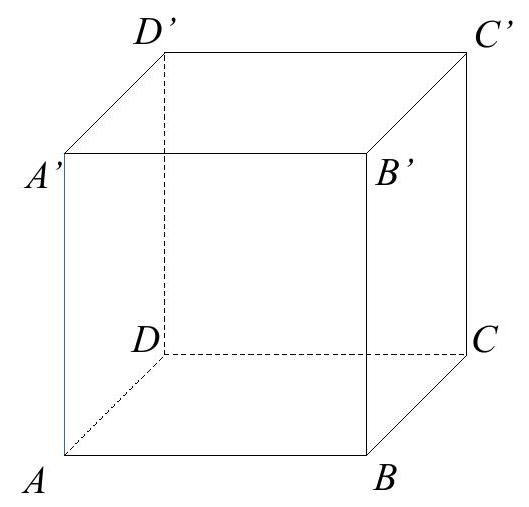
\includegraphics[max width=\textwidth, center]{2024_11_21_794e0c88574b53e7a852g-1}


\end{document}